\documentclass[11pt,letterpaper]{article}

%%%%% DOCUMENT METADATA %%%%%%%%%%%%%%%%%%%%%%%%%%%%%%%%%%%%%%%%%%%%%%%%%%%%%%%

\author{Jacob Thomas Errington}
\title{Probability notes}
\date{}

%%%%% PACKAGES %%%%%%%%%%%%%%%%%%%%%%%%%%%%%%%%%%%%%%%%%%%%%%%%%%%%%%%%%%%%%%%%

\usepackage[margin=2.0cm]{geometry}
\usepackage{amsmath,amssymb,amsthm}
\usepackage{hyperref}
\usepackage{environ}
\usepackage{tikz}

%%%%% TIKZ %%%%%%%%%%%%%%%%%%%%%%%%%%%%%%%%%%%%%%%%%%%%%%%%%%%%%%%%%%%%%%%%%%%%

\usetikzlibrary{graphs,arrows}
\tikzset{
    shorten >=1pt,
    >=stealth',
}

%%%%% THEOREM-LIKE ENVIRONMENTS %%%%%%%%%%%%%%%%%%%%%%%%%%%%%%%%%%%%%%%%%%%%%%%

% Actual theorem-like things
\newtheorem{thm}{Theorem}
\newtheorem{prop}{Proposition}
\newtheorem{lem}{Lemma}

% Definitions and examples use the "definition style", where the text is
% written in roman and not in italic.
\theoremstyle{definition}
\newtheorem{defn}{Definition}[section]
\newtheorem{eg}{Example}

% Remarks use the remark style, where the word "remark" is shown in a less
% invasive way.
\theoremstyle{remark}
\newtheorem{rem}{Remark}[section]

% Solutions to exercises
\makeatletter
\newenvironment{solution}{
    \let\oldqedsymbol=\qedsymbol%
    \def\@addpunct##1{}%
    \renewcommand{\qedsymbol}{$\blacktriangleleft$}%
    \begin{proof}[\textit Solution.]
}{
    \end{proof}%
    \renewcommand{\qedsymbol}{\oldqedsymbol}
}
\makeatother

% Memorized equation
% \NewEnviron{memequation}[1]{
%     \begin{equation}
%         \label{eq:#1}
%         \BODY
%     \end{equation}
% 
%     \expandafter\let\csname RecallBody#1\endcsname\BODY
%     \expandafter\gdef\csname Recall#1\endcsname{%
%         \begin{equation*}
%             \csname RecallBody#1\endcsname
%             \tag{recall \ref{eq:#1}}
%         \end{equation*}
%     }
% }

%%%%% MATHEMATICAL SHORTHANDS %%%%%%%%%%%%%%%%%%%%%%%%%%%%%%%%%%%%%%%%%%%%%%%%%

% Misc math operators
\newcommand{\parens}[1]{\left(#1\right)}
\newcommand{\abs}[1]{\left\lvert#1\right\rvert}
\newcommand{\setof}[1]{\left\{#1\right\}}
\newcommand{\Union}{\bigcup}
\newcommand{\union}{\cup}
\newcommand{\Intersn}{\bigcap}
\newcommand{\intersn}{\cap}
\newcommand{\symdiff}{\,\Delta\,}
\newcommand{\fact}{!\,}
\newcommand{\given}{\;\vert\;}
\newcommand{\compl}{^c}
\newcommand{\inv}{^{-1}}
\newcommand{\preimage}[1]{^{-1}\parens{\setof{#1}}}
\newcommand{\compose}{\circ}
\newcommand{\range}[2][1]{%
    \setof{#1,\ldots,#2}
}
\newcommand{\infsum}{\sum^\infty}
\renewcommand{\d}[2][]{%
    \ensuremath
    \frac{\mathrm{d}#1}{\mathrm{d}#2}
}

% Sets of numbers
\newcommand{\R}{\mathbb{R}}
\newcommand{\N}{\mathbb{N}}

% Probabilistic operators
\DeclareMathOperator{\Prob}{P}
\renewcommand{\P}[1]{\Prob{\parens{#1}}}
\DeclareMathOperator{\prob}{p}
\newcommand{\p}[2][]{%
    \def\temp{#2}
    \ifx\temp\empty
        \prob{\parens{#2}}
    \else
        \prob_{#1}{\parens{#2}}
    \fi
}
\DeclareMathOperator{\Expect}{\mathbb{E}}
\newcommand{\E}[1]{\Expect{\left[#1\right]}}
\DeclareMathOperator{\Var}{\mathbb{V}}
\newcommand{\V}[1]{\Var{\parens{#1}}}

% Distributions
\DeclareMathOperator{\BinOp}{Bin}
\newcommand{\Bin}[1]{ \BinOp\parens{#1} }

% Absolutely misc
\renewcommand{\th}{\textsuperscript{th}}

\begin{document}

\maketitle

\section{Miscellaneous analysis and combinatorics facts}

\begin{thm}{(Binomial expansion.)}
    \label{thm:binomial-expansion}
    For $x, y \in \R$ and any $n \in \N$
    \begin{equation}
        \label{eq:binomial-expansion}
        (x + y)^n = \sum_{k=0}^n {
            {n \choose k} x^k y^{n -k}
        }
    \end{equation}
\end{thm}

\begin{thm}{(Exponential series.)}
    \label{thm:exponential-series}
    For $x \in \R$,
    \begin{equation}
        \label{eq:series-ex}
        e^x = \infsum_{n=0} {
            \frac{x^n}{n\fact}
        }
    \end{equation}
\end{thm}

\begin{thm}{(Geometric series.)}
    \label{thm:geometric-series}
    For $x \in (-1, 1)$,
    \begin{equation}
        \label{eq:geometric-series}
        \frac{1}{1 - x} = \infsum_{n=0} { x^n }
    \end{equation}
\end{thm}

\begin{rem}
    \label{rem:differentiate-geometric-series}
    Both sides of \eqref{eq:geometric-series} may be differentiated to obtain
    other useful equalities involving series, e.g.
    \begin{equation*}
        \d{x}\parens{ \frac{1}{1-x} }
        =
        \parens{1-x}^{-2}
        =
        \infsum_{n=1} { n x^{n-1} }
    \end{equation*}
\end{rem}

\begin{thm}{(Negative binomial series.)}
    \label{thm:negative-binomial-series}
    For $n > 0$ and $x \in (-1, 1)$,
    \begin{equation}
        \label{eq:negative-binomial-series}
        (1+x)^{-n} = \infsum_{k=0} {
            {{n + k - 1} \choose k} (-1)^k x^k
        }
    \end{equation}
\end{thm}

\begin{defn}{(Limit definition of $e$.)}
    \label{def:limit-e}
    Suppose $\lim_{n\to\infty} x_n = x$. Then,
    \begin{equation}
        \label{eq:limit-e}
        \lim_{n\to\infty} {
            \parens{
                1 + \frac{x_n}{n}
            }^n
        }
        =
        e^x
    \end{equation}
\end{defn}

\begin{rem}
    If we use a constant sequence $(x_n)_{n\in\N}$, such that $x_n = \lambda$,
    in definition \ref{def:limit-e}, then
    \begin{equation*}
        \lim_{n\to\infty} {
            \parens{
                1 + \frac{\lambda}{n}
            }^n
        }
        =
        e^x
    \end{equation*}
\end{rem}

\begin{rem}{($e^x$ grows really fast.)}
    For any $a \in R$,
    \begin{equation*}
        \lim_{x\to\infty} {
            \frac{x^a}{e^x}
        }
        = 0
    \end{equation*}
\end{rem}

\section{Experiments, sample space, events, and probability}

\begin{defn}
    An \emph{experiment} is the process by which an observation is made. The
    set of all possible outcomes of an experiment forms the \emph{sample space}
    for the experiemnt. A subset of the sample space is called an \emph{event}.
\end{defn}

\begin{eg} ~

    \begin{enumerate}
        \item Measuring the lifetime of a bulb in a continuous time unit.

            The sample space is $S_1 = [0, \infty)$.
            The event $E_1 = [1000, 2000]$ corresponds to the lifetime being in
            between $1000$ and $2000$ units. (For example hours.)

        \item Rolling a die.

            The sample space is $S_2 = \{1,2,3,4,5,6\}$.
            $E_2 = \{3\}$ and $E_3 = \{2,4,6\}$ are examples of events.
    \end{enumerate}
\end{eg}

\begin{defn}
    An event that contains only one sample point, i.e. corresponds to a single
    outcome, is called a \emph{simple} event. An event that is not simple, i.e.
    corresponds to multiple outcomes, is a \emph{compound event}.
\end{defn}

\begin{defn}
    A \emph{probabilistic model} for an experiment with a discrete sample space
    $S = \{\omega_1, \omega_2, \ldots\}$
    can be identified with a function $p : S \to \R^+$, called the
    \emph{probability distribution}, which maps outcomes of the experiment to a
    nonnegative real number called that outcome's \emph{probability}.
\end{defn}

The intuitive interpretation of the probability of an outcome is that if we
repeat the outcome $n$ times and $n_\omega$ is the number of times that outcome
$\omega$ occurs, then $\lim_{n\to\infty} \frac{n_\omega}{n} = p(\omega)$.

\begin{defn}
    The \emph{probability} is a function $P : 2^S \to \R^+$ that assigns to
    each event in the sample space a nonnegative number.

    The probability is subject to the following laws.

    \begin{enumerate}
        \item $\forall E \subseteq S : \P{E} \geq 0$

            Negative probabilities are not allowed.

        \item $\P{S} = 1$

            Something has to happen.

        \item If $(A_i)_{i\in I}$ for $I \subseteq \N$ are pairwise disjoint
            events, then
            \begin{equation}
                \P{\Union_{i \in I} A_i} = \sum_{i \in I} \P{A_i}
                \label{eq:countable-additivity}
            \end{equation}

            The \emph{countable additivity} property. For a finite index set
            $I \subset \N$, it is called the \emph{finite additivity} property.
    \end{enumerate}
\end{defn}

\begin{rem}
    This definition of the probability function makes no explicit reference to
    discrete probability spaces. Indeed, it works for continuous spaces too, as
    we will see later.
\end{rem}

\begin{rem}
    For discrete probability spaces, the probability $P : 2^S \to \R^+$ is
    given by
    \begin{equation*}
        P(E) = \sum_{\omega \in E} p(\omega)
    \end{equation*}
\end{rem}

\begin{lem}
    Basic properties of probability.

    \begin{enumerate}
        \item Probability of subevents.
            \begin{equation*}
                A \subseteq B \implies \P{A} \leq \P{B}
            \end{equation*}

        \item Probability of the complement.
            \begin{equation*}
                \label{eq:complement-probability}
                \P{A^c} = 1 - \P{A}
            \end{equation*}

        \item Probability of the union.
            \begin{equation*}
                \P{A \union B} = \P{A} + \P{B} - \P{A \intersn B}
            \end{equation*}

        \item The union bound.
            \begin{equation}
                \label{eq:union-bound}
                \P{\Union_{i \in I} A_i} \leq \sum_{i \in I} \P{A_i}
            \end{equation}

        \item The law of excluded middle. (?)
            \begin{equation}
                \label{eq:excluded-middle}
                \P{A}
                = \P{A \intersn B} + \P{A \intersn B^c}
                = \P{A \intersn B} + \P{A \setminus B}
            \end{equation}
    \end{enumerate}
\end{lem}

\begin{rem}
    To compute the probability of an event in a discrete probability space, it
    suffies to sum the probabilities of all the outcomes in the event.
\end{rem}

\begin{rem}
    If the sample space $S$ is \emph{finite} and each outcome is
    \emph{equally likely}, then $\forall \omega \in S$, we have
    $\P{\{\omega\}} = \frac{1}{|S|}$. Hence, for any event $E \subseteq S$,
    \begin{equation*}
        \P{E} = \frac{|E|}{|S|}
    \end{equation*}
\end{rem}

\begin{eg}{(\#2.17 in the textbook.)}
    Products manufactured in a facility are tested for defects. Historical
    records indicate that $8\%$ of products have a type $A$ defect, $6\%$ have
    a type $B$ defect, and $2\%$ have both types of defects.

    If one item is chosen at random, what is the probability that
    \begin{enumerate}
        \item it has exactly one type of defect?
        \item it is \emph{not} defective?
    \end{enumerate}
\end{eg}

\begin{solution}
    Let $A$ denote the event that the item has a type $A$ defect.
    Likewise for $B$. Then, from the problem statement, we have that
    $\P{A} = 0.08$, $\P{B} = 0.06$, and $\P{A \intersn B} = 0.02$.

    \begin{enumerate}
        \item
            The event that the item has \emph{exactly one} type of defect is
            represented by
            \begin{equation*}
                A \symdiff B = (A \setminus B) \union (B \setminus A)
            \end{equation*}
            (This is the logical ``exclusive or''.)

            From the law of excluded middle \eqref{eq:excluded-middle}, we
            infer
            \begin{align*}
                \P{A \setminus B} &= \P{A} - \P{A \intersn B} \\
                \P{B \setminus A} &= \P{B} - \P{A \intersn B}
            \end{align*}

            Since $A \setminus B$ and $B \setminus A$ are disjoint, we can
            apply the finite additivity property in
            \eqref{eq:countable-additivity} to obtain
            \begin{align*}
                \P{A \symdiff B}
                &= \P{A \setminus B} + \P{B \setminus A} \\
                &= \P{A} + \P{B}- 2\P{A \intersn B} \\
                &= 0.08 + 0.06 - 2 \times 0.02 = 0.01
            \end{align*}

        \item
            The event that the item is \emph{not} defective is given by
            $(A \union B)^c$. We know that
            \begin{equation*}
                \P{A \union B}
                = \P{A} + \P{B} - \P{A \intersn B}
                = 0.08 + 0.06 - 0.02
                = 0.12
            \end{equation*}
            Then, from the probability of the complement
            \eqref{eq:complement-probability}, we compute
            \begin{equation*}
                \P{(A \union B)^c} = 1 - \P{A \union B} = 1 - 0.12 = 0.88
            \end{equation*}

    \end{enumerate}
\end{solution}

\section{Counting techniques}

This section presents the four basic rules of counting.

\subsection{Multiplication rule}
\label{sec:multiplication-rule}

Suppose there are two tasks to perform. If the first can be performed in $n$
ways and the second can be performed in $m$ ways, then jointly they can be
perform in $n \times m$ ways.

The multiplication rule extends inductively. It can also be used to see how
many ways there are of ordering $n$ items; this is
\begin{equation*}
    $n! = 1 \times 2 \times \cdots \times n$.
\end{equation*}

\subsection{Permutation rule}
\label{sec:permutation-rule}

Suppose we have $n$ distinct objects and $r$ distinct boxes into which we would
like to fit them. Each box may hold exactly one object, and $r \leq n$. Then,
the number of ways of filling up the boxes is
\begin{equation}
    \label{eq:permutation-rule}
    P_r^n = \frac{n!}{(n-r)!}
\end{equation}

\subsection{Selection rule}
\label{sec:selection-rule}

Suppose we want to select $r$ objects from a set of $n$ objects, where
$r \leq n$. The order of the selection doesn't matter. The number of ways to do
this is
\begin{equation}
    \label{eq:selection-rule}
    C_r^n = {n \choose r} = \frac{n\fact}{(n-r)\fact r\fact}
\end{equation}

Why is this? First apply the permutation rule. The number we get will be too
big, as we are counting each selection $r!$ times, one for each possible
arrangement of that selection. Hence, dividing by $r!$ corrects this
double-counting.

\subsection{Partition rule}
\label{sec:partition-rule}

Suppose we want to partition a set $S$ such that $|S| = n$ into $k$ groups,
with sizes $n_1, \ldots, n_k$ such that $\sum_{i=1}^k n_i = n$. The number of
ways to do this is
\begin{equation}
    \label{eq:partition-rule}
    {n \choose n_1 \, \cdots \, n_k}
    = \frac{n\fact}{n_1\fact \cdots n_k\fact}
\end{equation}

\begin{eg}
    Four people get into an elevator, and each of them can get off at one of
    $10$ floors. Assuming each person gets off a a random floor, what is the
    probability that no two get off at the same floor?
\end{eg}

\begin{solution}
    Let $S$ be the sample space and $E$ denote the event that no two get off at
    the same floor. Note that a person getting off at a certain floor does not
    restrict the choices of floors that others may get off at.
    Hence, $|S| = 10^4$. Each of the outcomes is equally likely.

    The event is that no two get off at the same floor, i.e. that they all get
    off on different floors. So if the first person gets off at some floor,
    then no others can get off there. Hence, each time someone gets off, a
    restriction occurs.
    \begin{equation*}
        |E| = P_4^{10} = 10 \times 9 \times 8 \times 7
    \end{equation*}

    The probability of this event is
    \begin{equation*}
        \P{E}
        = \frac{|E|}{|S|} = \frac{10 \times 9 \times 8 \times 7}{10^4}
        = 0.504
    \end{equation*}
\end{solution}

\begin{eg}
    A $5$-card poker hand is said to be a full house if it consists of $3$
    cards of the same denomination and $2$ other cards of the same
    denomination. These denominations must be different.

    If a $5$-card hand is dealt randomly, what is the probability that it is a
    full house?
\end{eg}

\begin{solution}
    The sample space is the set of all $5$-card hands, i.e. unordered choices
    of $5$ elements from a $52$-element set. Hence, $|S| = {52 \choose 5}$.

    Next, the event can be described by a sequence of choices. First, choose
    the denominations, which must be different. Second, choose the suits.
    \begin{equation*}
        |E| = (13 \times 12) \times \parens{{4 \choose 3} \times {4 \choose 2}}
    \end{equation*}

    The probability is therefore
    \begin{equation*}
        \P{E}
        = \frac{|E|}{|S|}
        = \frac{
            (13 \times 12) \times \parens{{4 \choose 3} \times {4 \choose 2}}
        }{
            {52 \choose 5}
        }
    \end{equation*}
\end{solution}

\section{Conditional probability}

\begin{defn}
    The \emph{multiplicative law of probability} is
    \begin{equation}
        \label{eq:multiplicative-law}
        \P{A \given B} \P{B} = \P{A \intersn B}
    \end{equation}

    From the multiplicative law, we can understand
    \emph{conditional probability}, when $\P{B} \neq 0$.
    \begin{equation}
        \label{eq:conditional-probability}
        \P{A \given B} = \frac{\P{A \intersn B}}{\P{B}}
    \end{equation}
\end{defn}

\begin{thm}{(Total probability.)}
    \label{thm:total-probability}
    If $\mathcal{S} = \{B_1, B_2, \ldots\}$ is a countable partition of a
    sample space $S$ such that $\P{B_i} > 0$ for all $i$, then for any event
    $A \subseteq S$,
    \begin{equation*}
        \P{A} = \sum_{i} \P{A \given B_i} \P{B_i}
    \end{equation*}
\end{thm}

\begin{rem}
    The Law of Excluded Middle (equation \ref{eq:excluded-middle}) is a special
    case of the Law of Total Probability (Theorem \ref{thm:total-probability}.)
    obtained by partitioning over $B$ and its complement $B^c$.
\end{rem}

\begin{proof}
    Note that $\setof{B, B^c}$ forms a partition of the sample space. Hence by
    applying the Law of Total Probability and the definition of conditional
    probability, we get
    \begin{align*}
        \P{A}
        &= \P{A \given B} \P{B} + \P{A \given B^c} \P{B^c} \\
        &= \frac{\P{A \intersn B}}{\P{B}} \P{B}
            + \frac{\P{A \intersn B^c}}{\P{B^c}} \P{B^c} \\
        &= \P{A \intersn B} + \P{A \intersn B^c}
    \end{align*}
\end{proof}

\begin{eg}
    \label{eg:marys-urns}
    Mary is given two urns. The first urn contains five red balls and three
    blue balls. The second urn contains 4 red balls and three blue balls. Mary
    chooses urn $1$ with probability $\frac{1}{3}$ and urn $2$ with probability
    $\frac{2}{3}$. Then, she selects one ball from the urn uniformly at random.

    What is the probability that the selected ball is red?
\end{eg}

\begin{solution}
    Let $U_1$ denote the event of choosing urn $1$, and $U_2$ for choosing urn
    $2$. Let $R$ denote the event that a red ball is selected.

    Notice that the sample space is partitioned according to the choice of urn,
    so we apply the total proabbility theorem.
    \begin{equation*}
        \P{R}
        = \P{R \given U_1}\P{U_1} + \P{R \given U_2}\P{U_2}
        = \frac{5}{8} \times \frac{1}{3} + \frac{4}{7} \times \frac{2}{3}
        = \frac{5}{24} + \frac{8}{21}
    \end{equation*}
\end{solution}

\begin{thm}{(Bayes.)}
    \label{thm:bayes}
    If $\mathcal{S} = \{B_1, B_2, \ldots\}$ is a countable partition of a
    sample space $S$ and $\P{B_i} > 0$, then for any event $A$ with
    $\P{A} > 0$,
    \begin{equation}
        \label{eq:bayes}
        \P{B_i \given A}
        = \frac{\P{A \given B_i}\P{B_i}}{\sum_{k} \P{A \given B_k} \P{B_k}}
    \end{equation}
\end{thm}

\begin{eg}
    In the same context as example \ref{eg:marys-urns}, if the selected ball
    turns out red, then what is the probability that urn $1$ was selected?
\end{eg}

\begin{solution}
    Using Bayes's theorem,
    \begin{equation*}
        \P{U_1 \given R}
        = \frac{\P{R \given U_1} \P{U_1}}{\P{R}}
        = \frac{\frac{5}{3} \times \frac{1}{3}}{\frac{5}{24} + \frac{8}{21}}
    \end{equation*}
\end{solution}

\section{Discrete random variables}

\begin{defn}
    A \emph{random variable} is a function defined on some sample space that
    takes values in $\R^d$.

    Concretely, if $S$ is a sample space, then $X : S \to \R^d$ is a random
    variable.
\end{defn}

\begin{defn}{(Discrete random variable.)}
    If the image $X(S)$ of a random variable $X : S \to \R^d$ is countable, the
    variable is said to be \emph{discrete}.
\end{defn}

\begin{rem}
    If $X$ is an $\R^d$-values random variable defined on a sample space $S$,
    then for any subset of its codomain $A \subseteq \R^d$,
    \begin{equation}
        \label{eq:random-variable-preimage}
        X\inv (A) = \{\omega \in S : X(\omega) \in A\}
    \end{equation}
    is an event.

    If $\Prob$ is a probability on $S$, then we write
    \begin{equation*}
        \P{X \in A}
    \end{equation*}
    to mean
    \begin{equation*}
        \P{\{\omega \in S : X(\omega) \in A\}}
    \end{equation*}
\end{rem}

\begin{rem}
    In the spirit of the previous remark, when the set $A$ is a singleton, we
    write $\P{X = x}$ to mean $\P{\{\omega \in S : X(\omega) = x\}}$.
\end{rem}

\begin{defn}{(Probability distribution.)}
    If $X : S \to \R^d$ is a discrete random variable defined on a sample space
    $S$ with associated probability $\Prob$ and we enumerate the image of $X$
    by $x_1, x_2, \ldots$, then the \emph{probability distribution} of $X$ is
    represented by the function $\prob : \R^d \to \R$ given by
    \begin{equation}
        \label{eq:probability-distribution}
        x_i \mapsto \P{X = x_i}
    \end{equation}
    for $i \in \N$.

    Intuitively, a probability distribution is an explicit characterization
    of the likelihood of each potential value of a random variable.

    The following diagram illustrates the relationship between the random
    variable $X$, the probability $\Prob$, and the probability distribution $p$
    of $X$.

    \begin{center}
        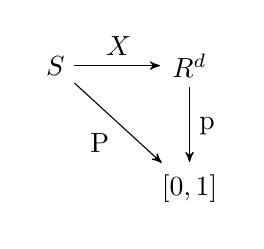
\begin{tikzpicture}
            \matrix[column sep=1cm, row sep=1cm]{
                \node (S) {$S$} ; & \node (Rd) {$R^d$} ; \\
                                  & \node (R) {$[0, 1]$} ; \\
            } ;
            \graph[use existing nodes]{
                S ->[edge label={$X$}]
                Rd ->[edge label={$\prob$}]
                R ;
                S ->[edge label={$\Prob$}, swap]
                R ;
            } ;
        \end{tikzpicture}
    \end{center}
\end{defn}

\begin{eg}
    A fair coin is tossed twice. Let $X$ be a random variable describing the
    number of tails. Find the distribution of $X$.
\end{eg}

\begin{solution}
    The possible values of $X$ are $0$, $1$, and $2$. Thus the distribution of
    $X$ is given by
    \begin{align*}
        \p{0} &= \P{X = 0} = \frac{1}{4} \\
        \p{1} &= \P{X = 1}
            = \P{HT} + \P{TH} = \frac{1}{4} + \frac{1}{4} = \frac{1}{2} \\
        \p{2} = \P{X = 2} = \P{TT} = \frac{1}{4}
    \end{align*}
\end{solution}

\begin{eg}
    \label{eg:distribution-of-until-6}
    Roll a fair die until a six appears. Let $X$ be the number of required
    tosses. Find the distribution of $X$.
\end{eg}

\begin{solution}
    Notice this time that the codomain of $X$ is countably infinite now. The
    possible values are $1,2,3,\ldots$. The distribution of $X$ is given by
    \begin{align*}
        \p{i} &= \P{X = i} \\
        &= \P{
            \Intersn_{k=1}^{i-1} \{
                \text{not $6$ in $k$\textsuperscript{th} toss}
            \}
            \intersn
            \{\text{$6$ in $i$\textsuperscript{th} toss}\}
        } \\
        &= \prod_{k=1}^{i-1} \P{\text{not $6$ in $k$\textsuperscript{th} toss}}
        \times \P{\text{$6$ in $i$\textsuperscript{th} toss}} \\
        &= \parens{\frac{5}{6}}^{i-1} \times \frac{1}{6}
    \end{align*}
\end{solution}

\begin{eg}
    Toss a fair coin and roll a fair die independently.
    Let
    \begin{equation*}
        X_1 = \begin{cases}
            0 &\quad\text{if toss is tails} \\
            1 &\quad\text{if toss is heads}
        \end{cases}
    \end{equation*}
    and $X_2$ be the value of the uppermost face of the die.

    Let $X = (X_1, X_2)$, so $X$ is an $\R^2$-valued random variable.
    What is the distribution of $X$?
\end{eg}

\begin{solution}
    Possible values of $X$ are
    \begin{equation*}
        (i, j) \in \{(i, j) : i \in \{0, 1\} \land j \in \range{6} \}
    \end{equation*}
    For any such $(i, j)$,
    \begin{equation*}
        \p{i, j}
        = \P{X = (i, j)}
        = \P{X_1 = i \land X_2 = j}
        = \P{X_1 = i} \times \P{X_2 = j}
        = \frac{1}{2} \times \frac{1}{6}
        = \frac{1}{12}
    \end{equation*}
\end{solution}

\begin{eg}
    A single cell can either die, with probability $0.1$, or split into two
    cells, with probability $0.9$, resulting in a new generation of cells. Each
    cell in the new generation dies or splits independently with the same
    probabilities. Supposing we start at generation zero with one cell and let
    it split or die to produce cells in generation one, what is the
    distribution of the number of cells in generation two?
\end{eg}

\begin{solution}
    Let $X_1$ be the number of cells in generation $1$. We have
    \begin{align*}
        \P{X_1 = 0} &= 0.1 \\
        \P{X_1 = 2} &= 0.9
    \end{align*}
    Let $X_2$ be the number of cells in generation $2$. We have
    \begin{align*}
        \P{X_2 = 0 \given X_1 = 0} &= 1 \\
        \P{X_2 = 2 \given X_1 = 0} &= 0 \\
        \P{X_2 = 4 \given X_1 = 0} &= 0 \\
        \P{X_2 = 0 \given X_1 = 2} &= 0.1 \times 0.1 \\
        \P{X_2 = 2 \given X_1 = 2} &= 0.1 \times 0.9 + 0.9 \times 0.1 \\
        \P{X_2 = 4 \given X_1 = 2} &= 0.9 \times 0.9
    \end{align*}

    Notice that $X_1 = 0$ and $X_1 = 2$ partition the space.
    Then by the total probability theorem \eqref{thm:total-probability},
    \begin{align*}
        \P{X_2 = 0}
        &= \P{X_2 = 0 \given X_1 = 0} \times \P{X_1 = 0}
        + \P{X_2 = 0 \given X_1 = 2} \times \P{X_1 = 2} \\
        &= 1 \times 0.1 + (0.1)^2 \times 0.9 \\
        \\
        \P{X_2 = 2}
        &= \P{X_2 = 2 \given X_1 = 0} \times \P{X_1 = 0}
        + \P{X_2 = 2 \given X_1 = 2} \times \P{X_1 = 2} \\
        &= 0 \times 0.1 + (2 \times 0.1 \times 0.9) \times 0.9 \\
        \\
        \P{X_2 = 4}
        &= \P{X_2 = 4 \given X_1 = 0} \times \P{X_1 = 0}
        + \P{X_2 = 4 \given X_1 = 2} \times \P{X_1 = 2} \\
        &= 0 \times 0.1 + (0.9)^2\times 0.9
    \end{align*}
\end{solution}

\subsection{Functions of random variables}

\begin{defn}
    \label{def:function-rv}
    If $X : S \to \R^m$ is a random variable and $g : \R^m \to \R^n$ is a
    function, then $Y = g \compose X$, often written $Y = g(X)$, is an
    $\R^n$-valued random variable.
\end{defn}

\begin{rem}
    If the possible values of $X : S \to \R^m$ are enumerated
    $\setof{x_1, x_2, \ldots}$ and $\p[X]{x_i}$, $i = 1,2,\ldots$ is the
    distribution of $X$, then the distribution of
    $Y = g \compose X : S \to \R^n$ can be computed by
    \begin{enumerate}
        \item
            Enumerating the image of $Y$ by $\setof{y_1, y_2, \ldots}$.

        \item
            For each $j$, find the preimage of $y_j$ under $g$ to recover
            subsets of the image of $X$.
            \begin{equation*}
                E_j = \{ x \in \{x_1, \ldots\} : g(x) = y_i \}
            \end{equation*}

        \item
            The distribution of $Y$ is given by
            \begin{align}
                \p[Y]{y_j} &= \sum_{x \in E_j} {\p[X]{x}} \notag \\
                \p[Y]{y_j} &= \sum_{x \in g\preimage{y_j}} {\p[X]{x}}
                \label{eq:pmf-of-composite-rv}
            \end{align}
            for $j = 1,2,\ldots$.
    \end{enumerate}
\end{rem}

\begin{eg}{(Square of a variable.)}
    Consider the sample space of outcomes of two dice rolls, so
    $S = \setof{(x, y) : x \in \range{6}, y \in \range{6}}$.
    We have a random variable $X$ that sums the pair and subtracts seven.
    \begin{equation*}
        X(x, y) = x + y - 7
    \end{equation*}
    Notice that the image $X(S) = \range[-5]{5}$.
    Consider the function $g : \R \to \R$ such that $x \mapsto x^2$.
    Let $Y : S \to \R$ be a random variable such that $Y = g(X)$.
    Find the probability distribution of $Y$ (i.e. of $X^2$).
\end{eg}

\begin{solution}
    First, we look at the image of $Y$.
    It is the set of squares of the numbers $\range[0]{5}$,
    i.e.  $\setof{0, 1, 4, 9, 16, 25}$.
    Notice that the preimage of each singleton has exactly two elements, except
    in the case of $0$. Then, we apply \eqref{eq:pmf-of-composite-rv} on each
    preimage to find the probability distribution of the transformed random
    variable.

    \begin{center}
        \begin{tabular}{c c c}
            $y \in Y(S)$ & $g\preimage{y}$ & $\p[Y]{y}$\\ \hline
            $0$          & $\setof{0}$     & $6/36$ \\
            $1$          & $\setof{-1,1}$  & $10/36$ \\
            $4$          & $\setof{-2,2}$  & $8/36$ \\
            $9$          & $\setof{-3,3}$  & $6/36$ \\
            $16$         & $\setof{-4,4}$  & $4/36$ \\
            $25$         & $\setof{-5,5}$  & $2/36$
        \end{tabular}
    \end{center}

    To see that indeed $\p[Y]{1} = \frac{10}{36}$ for instance,
    notice that $\p[X]{-1} = \frac{5}{36}$, as $X = -1$ occurs when we roll a
    sum of $6$.
    Such a sum being rolled can occur in $5$ ways,
    as $\abs{\setof{(6 - i, i) : i \in \range{5}}} = 5$,
    and there are a total of $36$ possible rolls of two dice.
    A symmetrical applies to rolling a sum of $8$, which in turn produces the
    value of the random variable $X = 1$.
    Hence $\p[Y]{1} = \p[X]{-1} + \p[X]{1} = \frac{5}{36} + \frac{5}{36}$.
\end{solution}

\subsection{Expectation of a random variable}

\begin{defn}
    \label{def:expectation}
    Let $X$ be a discrete random variable with enumerated image $x_1, \ldots$
    and probability distribution $\prob{x_i}$, for $i = 1,\ldots$.
    The \emph{expectation} of a $X$ is given by
    \begin{equation*}
        \E{X} = \sum_i x_i \p{x_i}
    \end{equation*}
\end{defn}

\begin{rem}
    If $X$ is $\R^d$-valued, then $\E{X} \in \R^d$, since $\p{x_i}$ is a
    scalar.
\end{rem}

\begin{defn}
    Suppose $X$ is a real-valued random variable and denote by $x_1^+,\ldots$
    and $x_1^-,\ldots$ the positive and negative values assumed by $X$,
    respectively.
    The expectation $\E{X}$ is defined \emph{only} when one of
    \begin{align*}
        \sum_i x_i^+ \p{x_i^+} &< \infty \\
        \sum_i x_i^- \p{x_i^-} &< \infty
    \end{align*}
    holds.
    If both these quantities are infinite, then we say that the expectation
    $\E{X}$ \emph{does not exist}.

    Similar considerations apply for vector-valued random variables
\end{defn}

\begin{eg}
    Roll a fair die until $6$ appears and let $X$ be the number of required
    tosses. What is the expectation of $X$?
\end{eg}

\begin{solution}
    Recall from example \ref{eg:distribution-of-until-6} the
    distribution of $X$
    \begin{equation*}
        \p{i} = \parens{\frac{5}{6}}^{i-1} \times \frac{1}{6}
    \end{equation*}

    Using this distribution, we compute the expectation of $X$
    \begin{align*}
        \E{X}
            &= \sum_{i} i \times \parens{\frac{5}{6}}^{i-1} \times \frac{1}{6} \\
            &= \frac{1}{6} \times \frac{1}{\parens{1 - \frac{5}{6}}^2} \\
            &= \frac{1}{6} \times 36 = 6
    \end{align*}
\end{solution}

\begin{thm}{(Linearity of expectation.)}
    Suppose $X$ is an $\R^m$-valued discrete random variable
    and $g_i : \R^m \to \R^n$ for $i \in \range{k}$. Then,
    \begin{equation*}
        \E{g_1(X) + \cdots + g_k(X)}
        = \E{g_1(X)} + \cdots + \E{g_k(X)}
    \end{equation*}
\end{thm}

\begin{rem}{(Expectation of a constant.)}
    Constant values are non-random. Hence, their expectation is simply their
    value. Formally, suppose $a \in \R$. Then,
    \begin{equation*}
        \E{a} = a
    \end{equation*}
\end{rem}

\begin{proof}{(Of remark.)}
    To see this, notice that we can model a constant as a random variable
    taking on the constant value with probability $1$ and every other value
    with probability $0$. Then, the sum for the expectation degenerates into
    the constant value itself.
\end{proof}

\begin{thm}{(Expectation of a function of a discrete random variable.)}
    \label{thm:expectation-function-rv}
    Suppose $X : S \to A \subseteq \R^m$ is a random variable with probability
    distribution $\prob_X : A \to [0,1]$.
    Let $f : A \to B \subseteq \R^n$ be a function transforming the of the
    random variable $X$ into the variable $Y = f(X)$.
    (See definition \ref{def:function-rv}.)
    The expectation $\E{f(X)}$ is found by
    \begin{equation}
        \label{eq:expectation-function-rv}
        \E{Y}
        = \E{f(X)}
        = \sum_{x \in X} {
            f(x) \p[X]{x}
        }
    \end{equation}
\end{thm}

\begin{eg}
    Let $X$ be the number of times heads appears when a (possibly unfair) coin
    is tossed $n$ times. Suppose that the probability of landing heads in a
    single toss is $p$. Find $\E{X}$.
\end{eg}

\begin{solution}
    Notice that the sample space consists of $n$-tuples, each component of
    which being boolean.
    Let $X_i = 1_{A_i}$ be an indicator random variable, taking the value $1$
    when $s \in S$ is such that $s \in A_i$, where $A_i$ denotes the event that
    the $i$\th{} component of the tuple is $H$, i.e. the $i$\th{} toss comes up
    heads.
    Notice that the expectation of an individual toss degenerates into a
    probability
    \begin{equation*}
        \E{X_i}
        = \sum_{s \in S} {
            X_i(s) \p[X_i]{s}
        }
        = 1 \times p + 0 \times (1-p)
        = p
    \end{equation*}
    We can do this simplification of the sum because the random variable only
    looks at the $i$\th{} component of the component $s$. This component is
    either heads with probability $p$ or tails with probability $1 - p$.

    But then, the total number of heads is exactly $X = \sum_i^n X_i$, so by
    linearity of expectation, we have
    \begin{equation*}
        \E{X} = \sum_i^n { \E{X_i} } = np
    \end{equation*}
\end{solution}

\begin{thm}{(Expectation of a series.)}
    \label{thm:expectation-series}
    If each $X_i$ is a nonnegative real-valued random variable defined on the
    same sample space, then
    \begin{equation}
        \label{eq:expectation-series}
        \E{\sum_{i=0}^\infty {X_i}} = \sum_{i=0}^\infty {\E{X_i}}
    \end{equation}
\end{thm}

\begin{eg}
    If $X$ is a real-valued discrete random variable taking values in
    $\N = \setof{0, 1, 2, \ldots}$, then
    \begin{equation*}
        \E{X} = \sum_{k=1}^\infty \P{X \geq k}
    \end{equation*}
\end{eg}

\begin{solution}
    \newcommand{\Xgeq}[1]{\ensuremath \setof{X \geq #1}}
    \newcommand{\indicator}[1]{\ensuremath 1_{\Xgeq{#1}}}
    Notice that we can rewrite $X$ as a sum of indicator random variables.
    \begin{align*}
        X
        &= \indicator{1} + \indicator{2} + \cdots \\
        &= \sum_{i=1}^\infty { \indicator{i} }
    \end{align*}
    Notice that for an individual variable $\indicator{k}$ we have
    \begin{align*}
        \E{\indicator{k}}
        &= 0 \times \p[\indicator{k}]{0}
            + 1 \times \p[\indicator{k}]{1} \\
        &= \p[\indicator{k}]{1} \\
        &= \P{\Xgeq{k}}
    \end{align*}
    Each variable is nonnegative, so we apply the linearity of expectation.
    \begin{equation*}
        \E{X}
        = \sum_{k=1}^\infty {
            \E{\indicator{k}}
        }
        = \sum_{k=1}^\infty {
            \P{\Xgeq{k}}
        }
    \end{equation*}
    as required.
\end{solution}

\subsection{Variance of a random variable}

\begin{defn}{(Variance.)}
    \label{def:variance}
    Suppose $X : S \to \R$ is a real-valued random variable such that
    $\E{X^2} < \infty$.
    Then, the \emph{variance} of $X$ is
    \begin{equation}
        \label{eq:variance}
        \V{X} = \E{\parens{X - \E{X}}^2}
    \end{equation}
\end{defn}

\begin{defn}{(Standard deviation.)}
    \label{def:stdev}
    The \emph{standard deviation} $\sigma_X$ of a random variable
    $X : S \to \R$ is defined
    \begin{equation}
        \label{eq:stdev}
        \sigma_X = \sqrt{\V{X}}
    \end{equation}
\end{defn}

\begin{rem}
    By definition, the square of the standard deviation is the variance, so we
    often write $\sigma_X^2$ for $\V{X}$.
\end{rem}

\begin{thm}
    \label{thm:alternative-variance}
    For any random variable $X : S \to \R$,
    \begin{equation*}
        \V{X} = \E{X^2} - \E{X}^2
    \end{equation*}
\end{thm}

\begin{proof}
    \begin{align*}
        \V{X}
        &= \E{\parens{X - \E{X}}^2} \\
        &= \E{X^2 - 2 \cdot X \cdot \E{X} + \E{X}^2} \\
        &= \E{X^2} - 2 \E{X} \E{X} + \E{X}^2 \\
        &= \E{X^2} - \E{X}^2
    \end{align*}
\end{proof}

\begin{thm}{(Properties of variance.)}
    \label{thm:variance-properties}
    Suppose $X : S \to \R$ is a real-valued random variable. Then,
    \begin{enumerate}
        \item
            Suppose $a, b \in \R$. Then
            \begin{equation}
                \label{eq:variance-linearity}
                \V{a X + b} = a^2 \V{X}
            \end{equation}
    \end{enumerate}
\end{thm}

\begin{proof}
    \begin{enumerate}
        \item
            Let $Y = a X + b$ be a derived real-valued random variable.
            Then, $\E{Y} = a \E{X} + b$ and
            \begin{equation*}
                Y - \E{Y} = a(X - \E{X})
            \end{equation*}
            Hence,
            \begin{align*}
                \V{Y}
                &= \E{\parens{a\parens{X - \E{X}}}^2} \\
                &= a^2 \E{\parens{X - \E{X}}^2} \\
                &= a^2 \V{X}
            \end{align*}
    \end{enumerate}
\end{proof}

\begin{rem}
    In theorem \ref{thm:variance-properties},
    an intuitive notion is captured by \eqref{eq:variance-linearity}:
    uniformly \emph{shifting} a random variable (adding a constant) does
    not affect the variance, which can be thought of as a measure of how
    dispersed they are.
\end{rem}

\begin{eg}
    Suppose $X : S \to N = \range{n}$ is a discrete random variable
    with uniform probability distribution,
    i.e. $\p[X](i) = \frac{1}{n}$ for all $i \in N$.
    Find $\E{X}$ and $\sigma_X$.
\end{eg}

\begin{solution}
    Using definition \ref{def:expectation}, we compute $\E{X}$ and $\E{X^2}$.
    \begin{equation}
        \label{eq:expectation-discrete-uniform}
        \E{X}
        = \sum_{i = 1}^n {i \frac{1}{n}} = \frac{1}{n} \frac{n(n+1)}{2}
        = \frac{n+1}{2}
    \end{equation}

    Note that $\E{X}^2 = \frac{n^2}{4} + n + 1$.

    Next we compute $\E{X^2}$ in order to compute $\V{X}$.
    \begin{equation*}
        \E{X^2}
        = \sum_{i = 1}^n {i^2 \frac{1}{n}}
        = \frac{1}{n} \frac{n(n+1)(2n+1)}{6}
        = \frac{(n+1)(2n+1)}{6}
    \end{equation*}
    \newcommand{\expectXsq}{\ensuremath \frac{(n+1)(2n+1)}{6}}

    Using theorem \ref{thm:alternative-variance}, we compute the variance
    \begin{align*}
        \V{X}
        &= \E{X^2} - \E{X}^2 \\
        &= \frac{(n+1)(2n+1)}{6} - \frac{\parens{n+1}^2}{4} \\
        &= \frac{n+1}{12}\parens{
            2(2n + 1) - 3(n + 1)
        } \\
        &= \frac{n+1}{12}\parens{
            4n + 1 -3n - 3
        } \\
        &= \frac{n+1}{12}\parens{
            n - 1
        } \\
        &= \frac{n^2 - 1}{12}
    \end{align*}
    Then the standard deviation is the square root of this quantity.
    \begin{equation}
        \label{eq:variance-discrete-uniform}
        \sigma_X = \sqrt{
            \frac{n^2 - 1}{12}
        }
    \end{equation}
\end{solution}

\begin{rem}
    Applying \eqref{eq:expectation-discrete-uniform} and
    \eqref{eq:variance-discrete-uniform} we can easily find the expectation and
    standard deviation, respectively, of $X : S \to \range{6}$ representing the
    upper face of a roll of a fair die.
    (So $S = \range{6}$ as well and $X$ is the identity.)
    \begin{align*}
        \E{X}
        &= \frac{6 + 1}{2} = \frac{7}{2} \\
        %
        \sigma_X
        &= \sqrt{
            \frac{6^2 - 1}{12}
        }
        = \sqrt{ \frac{35}{12} }
    \end{align*}
\end{rem}


\end{document}
